\chapter{Experimental results and analysis}


\section{Final experimental setup and aggregation}

The main experimental question is whether Nystr\"om approximation can keep the prediction error close to full KRR while reducing runtime. The Superconductivity dataset remains the main experimental example, while two additional regression datasets are used in Section \ref{sec:additional_datasets} to determine whether the observed behaviour is specific to one kernel matrix.

\begin{table}[H]
\centering
\begin{tabular}{lccc}
\hline
Dataset & Available observations & Input features & Target \\
\hline
Superconductivity & $21\,263$ & $81$ & critical temperature \\
CASP protein structure & $45\,730$ & $9$ & RMSD \\
CT Slice Localization & $53\,500$ & $384$ & relative axial location \\
\hline
\end{tabular}
\caption{Regression datasets used in the final experiments.}
\label{tab:final_datasets}
\end{table}

All three datasets were obtained from the UCI Machine Learning Repository \citep{superconductivty_data_464, physicochemical_properties_of_protein_tertiary_structure_265, relative_location_of_ct_slices_on_axial_axis_206}. The patient identifier in the CT dataset was excluded from the input features.

For every dataset, we used $19\,000$ observations for training and $1\,000$ for testing. The train/test split was generated once and kept fixed throughout all five repetitions. The input features were standardized using the mean and standard deviation of the training data. The Gaussian RBF kernel
\[
k(x,z)=\exp(-\gamma\|x-z\|_2^2)
\]
was used with $\gamma=\frac{1}{d},$ where $d$ is the number of input features. The KRR regularization parameter was fixed at $\lambda_{\mathrm{KRR}}=0.01$, which gave a test MSE very close to or at the minimum of a preliminary parameter sweep for all three datasets.

The methods compared were full KRR, uniform Nystr\"om sampling, approximate leverage
score sampling and recursive ridge leverage score (RLS) sampling. For uniform and
approximate leverage sampling, the tested column counts were
\[
l\in\{50,100,200,400,800,1600\}.
\]
The approximate leverage sampling used an initial uniform sample of
\[
l_0=\min\{100,\max(1,\lfloor l/2\rfloor)\}.
\]
For recursive RLS, the tested parameters were
\[
\lambda_{\mathrm{RLS}}
\in\{1000,2000,5000,10000,20000\},
\qquad
\delta=0.1.
\]
The actual number of returned columns is random for recursive RLS because the method samples each point with probability $p_i$.

Each randomized method was run five times. The train/test split and all deterministic parameters were fixed while the randomized column selection was independently redrawn. For every metric, we computed the empirical mean, sample variance and sample standard deviation. The figures display the empirical mean with bars of one sample standard deviation. Recursive RLS is plotted at its mean selected column count and therefore has horizontal bars as well as vertical bars.

The full KRR solution does not change between repetitions because the split and parameters are fixed. Its dense solve and test prediction runtime was nevertheless repeated five times to obtain a stable mean solve time. The full KRR total reference time was obtained by adding the construction time of the full training and testing kernel matrices to the mean solve time.

The first metric is the relative kernel approximation error
\[
\frac{\|K-\tilde K\|_F}{\|K\|_F}.
\]
This measures how well the matrix $K$ itself is approximated. The second metric is the relative coefficient error
\[
\frac{\|\alpha-\tilde\alpha\|_2}{\|\alpha\|_2},
\]
where $\alpha$ is the full KRR solution and $\tilde\alpha$ is the approximate Nystr\"om solution. The third metric and the most important metric is test prediction error, measured by MSE and RMSE. The RMSE is especially useful in the final discussion because it is in the original units of the target variable \citep{cortes2010impact}.

To compare prediction error directly with the full KRR baseline, the relative excess test RMSE is defined as
\[
\frac{\mathrm{RMSE}_{\mathrm{approx}}-\mathrm{RMSE}_{\mathrm{full}}}{\mathrm{RMSE}_{\mathrm{full}}}.
\]
A value of zero means that the approximation matches the full KRR test RMSE. A value of $0.1$ means that the approximation has about $10\%$ larger RMSE than full KRR.

Runtime is split into sampling time and solve time. Sampling time measures the cost of choosing columns. Solve time includes constructing $C$ and $W$, computing the
factorized Nystr\"om approximation, solving for $\tilde{\alpha}$ and producing
the test predictions. Total time is the sum of these two. This distinction matters because, as we will see, the sampling step is not the main bottleneck once $l$ is moderately large. We now talk about the core results of this project.

\section{Prediction error against sampled columns}

We first look at prediction error as a function of the number of sampled columns. This is the most direct way to see whether Nystr\"om prediction moves toward full KRR as $l$ increases.

\begin{figure}[H]
\centering
\begin{minipage}{0.49\textwidth}
\centering
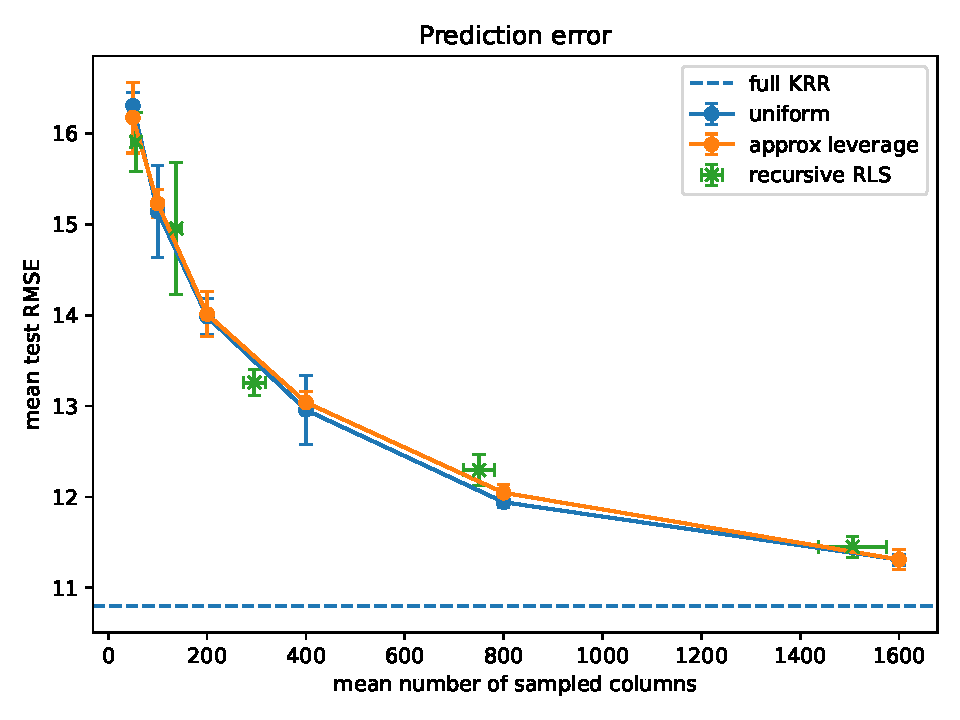
\includegraphics[width=0.98\textwidth]{Results/Superconductivityfinal_test_rmse_vs_l.pdf}
\caption{Mean test RMSE against mean $l$.}
\label{fig:ftrvl}
\end{minipage}
\hspace{0.005\textwidth}
\begin{minipage}{0.49\textwidth}
\centering
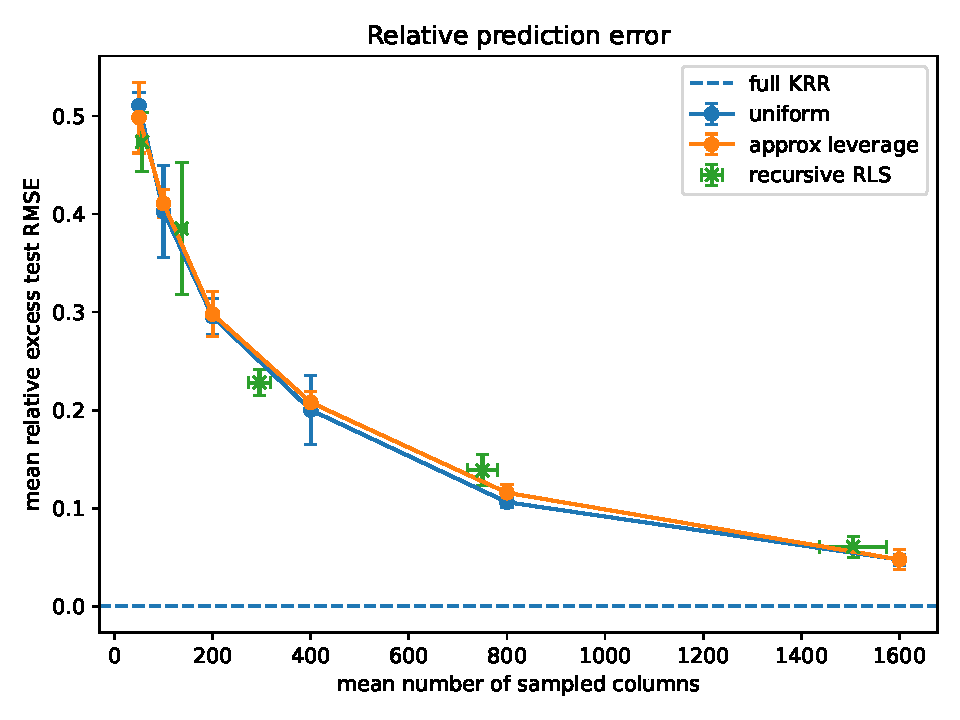
\includegraphics[width=0.98\textwidth]{Results/Superconductivityfinal_relative_excess_rmse_vs_l.pdf}
\caption{Mean relative excess test RMSE against mean $l$.}
\label{fig:frervl}
\end{minipage}
\end{figure}
\FloatBarrier

Figure \ref{fig:ftrvl} shows that the mean test RMSE decreases as more columns are sampled. This is as expected by theory \citep{cortes2010impact,bach2013sharp}, $\tilde K$ captures more information of $K$ with more columns, and the approximate KRR prediction becomes closer to the full KRR prediction. For the current experiments, the Nystr\"om curves approach this line, but they do not reach it for the tested values of $l$. This is a limitation of the tested landmark range but we see in the relative excess RMSE plot that the gap is small for the largest $l$ in figure \ref{fig:frervl}. At $l\approx1600$, all methods have a mean test RMSE of approximately $11.1$, compared with around $10.9$ for full KRR.

Uniform and approximate leverage sampling are very close. Approximate leverage is not consistently better even though it is more informed than uniform sampling theoretically. As we have seen before this may be due to the large amount of noise in the approximate scores compared to exact scores. Recursive RLS follows the same general trend, but its points are not on the same fixed-$l$ grid because the method chooses a random number of columns through its sampling probabilities.

The prediction error bars are small compared to the improvement achieved by increasing $l$. Therefore the decreasing error pattern is stable across the five column selections and is not caused by one particularly good or bad sample. The error bars and error curves of all methods are also similar for much of the tested range, so the repeated experiment does not show a consistent prediction advantage for approximate leverage sampling or recursive RLS sampling.

Figure \ref{fig:frervl} gives the same prediction result relative to the full KRR baseline. It makes the practical interpretation clearer as small values of $l$ are much worse than full KRR, while larger values reduce the gap. For uniform sampling, the mean relative excess RMSE decreases from approximately $51\%$ at $l=50$ to $20\%$ at $l=400$, $11\%$ at $l=800$ and $5\%$ at $l=1600$. Approximate leverage sampling and recursive RLS sampling follow almost the same curve. The relative excess RMSE for the largest fixed column count is small compared with the low columns cases. Thus the important question is not only whether increasing $l$ improves prediction, but also if the decrease in test error is worth the runtime.

\section{Runtime and prediction trade off}

In this section we investigate the runtime and prediction trade off. This is the central practical objective and the next figures are therefore the main results of the project.

\begin{figure}[H]
\centering
\begin{minipage}{0.49\textwidth}
\centering
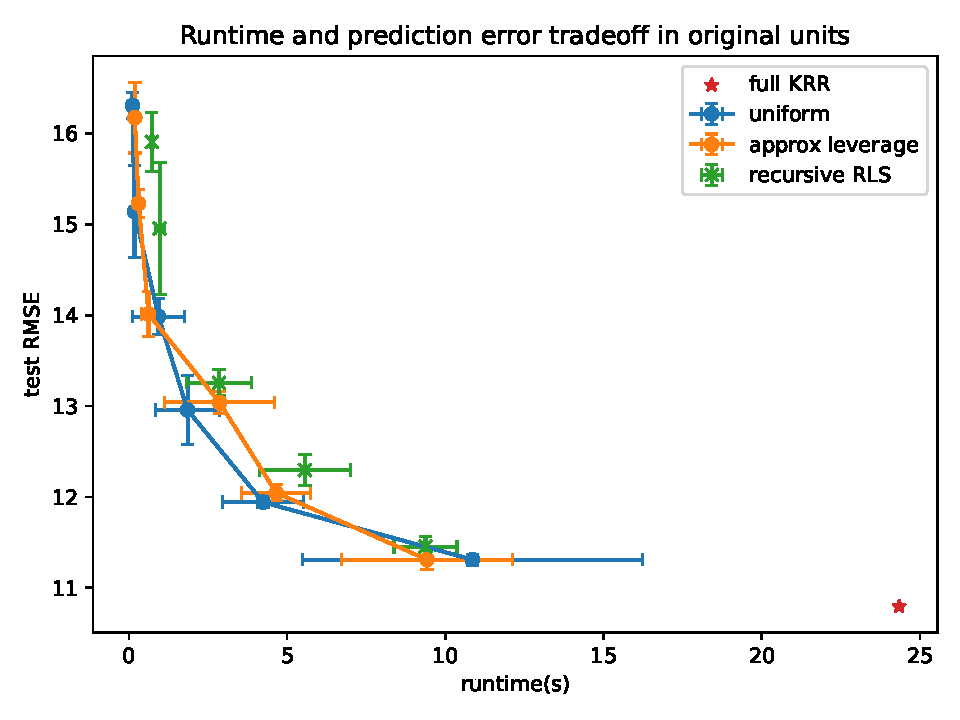
\includegraphics[width=0.78\textwidth]{Results/Superconductivityfinal_runtime_test_rmse_tradeoff.pdf}
\caption{Mean runtime and test RMSE trade off.}
\label{fig:frtr}
\end{minipage}
\hspace{0.005\textwidth}
\begin{minipage}{0.49\textwidth}
\centering
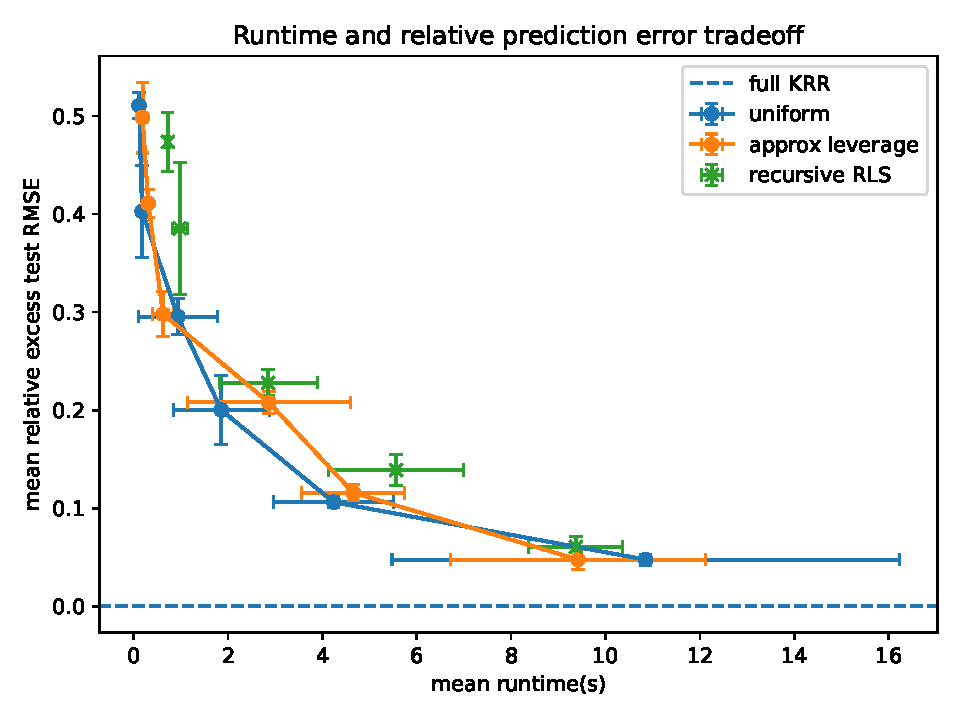
\includegraphics[width=0.78\textwidth]{Results/Superconductivityfinal_runtime_relative_excess_rmse_tradeoff.pdf}
\caption{Mean runtime and relative excess test RMSE compared with full KRR.}
\label{fig:rrer}
\end{minipage}
\end{figure}
\FloatBarrier

Figure \ref{fig:frtr} is the main prediction against runtime figure. It shows that all Nystr\"om methods improve as runtime increases, but the best prediction errors occur only at the larger tested runtimes. The full KRR reference point has the lowest RMSE. The Nystr\"om methods approach it, but the runtime advantage becomes smaller when there is a high number of columns selected. Although the runtime advantage narrows as $l$ increases, the largest tested Nystr\"om points still use less than half of the full KRR total reference time.

Figure \ref{fig:rrer} gives a clear normalized view of the same result. A value of zero means full KRR prediction accuracy. Values above zero measure how much worse the Nystr\"om method is in RMSE compared to full KRR. The plot shows a clear saturation pattern where the first increases in runtime give large prediction improvements, but the last part of the gap to full KRR is expensive. The elbow of the curve is around $0.1$ relative excess RMSE and approximately $4$--$5$ seconds runtime, which means that the Nystr\"om methods have about $10\%$ larger RMSE than full KRR using around one fifth of the runtime. In this experiment, this provides a reasonable trade off even though it still accepts a noticeable prediction loss. Increasing the fixed column count to $l=1600$ reduces the relative excess RMSE to approximately $5\%$, but raises the mean runtime to approximately $11$ seconds for uniform sampling and $9.5$ seconds for approximate leverage sampling. Thus roughly doubling the runtime only halves the remaining excess RMSE from approximately $10\%$ to $5\%$. This quantifies the diminishing returns near the full KRR solution. Of course, this is only one main dataset and one set of algorithms. Other datasets may have different trade offs as investigated in Section 5.6. 

\section{Runtime analysis and solver behaviour}

If we compare the previous plots on runtime and columns, we see that the runtime increases quickly with $l$. Specifically, at $l\approx1500$--$1600$, the time has already reached around $40\%$ of the mean full KRR total reference time. The question is why the runtime behaves this way. The next two figures show the sampling time and total time against $l$. The possible reason is that the sampling step itself is not the main bottleneck. Once the columns have been selected, all methods pass those columns to the same factorization solver.

\begin{figure}[H]
\centering
\begin{minipage}{0.49\textwidth}
\centering
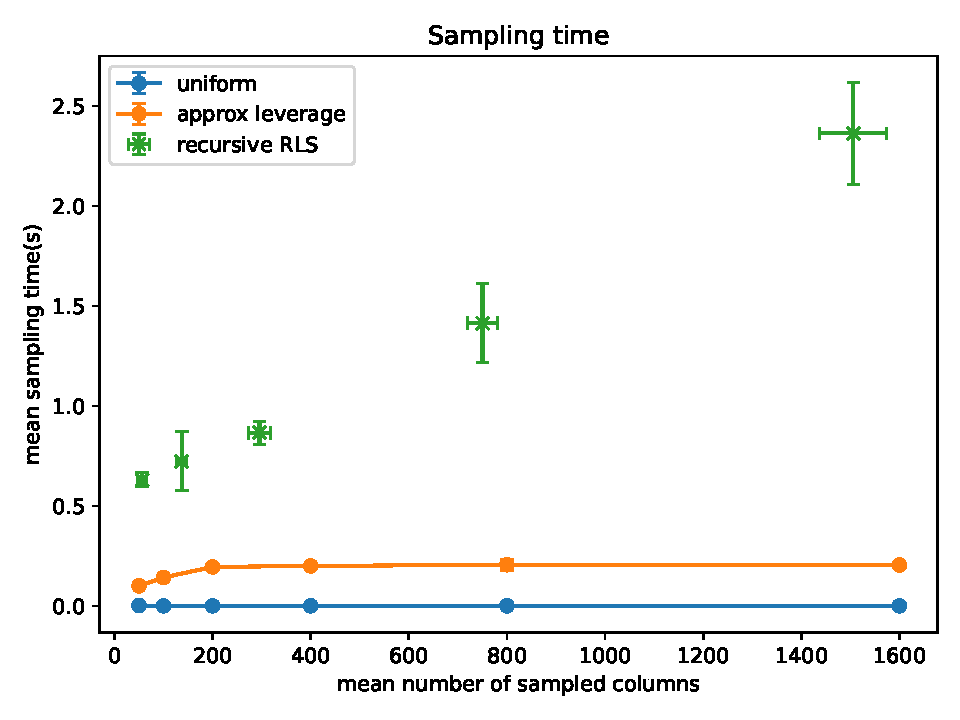
\includegraphics[width=0.98\textwidth]{Results/Superconductivityfinal_sample_time_vs_l.pdf}
\caption{Mean sampling time against mean $l$.}
\label{fig:fst}
\end{minipage}
\hspace{0.005\textwidth}
\begin{minipage}{0.49\textwidth}
\centering
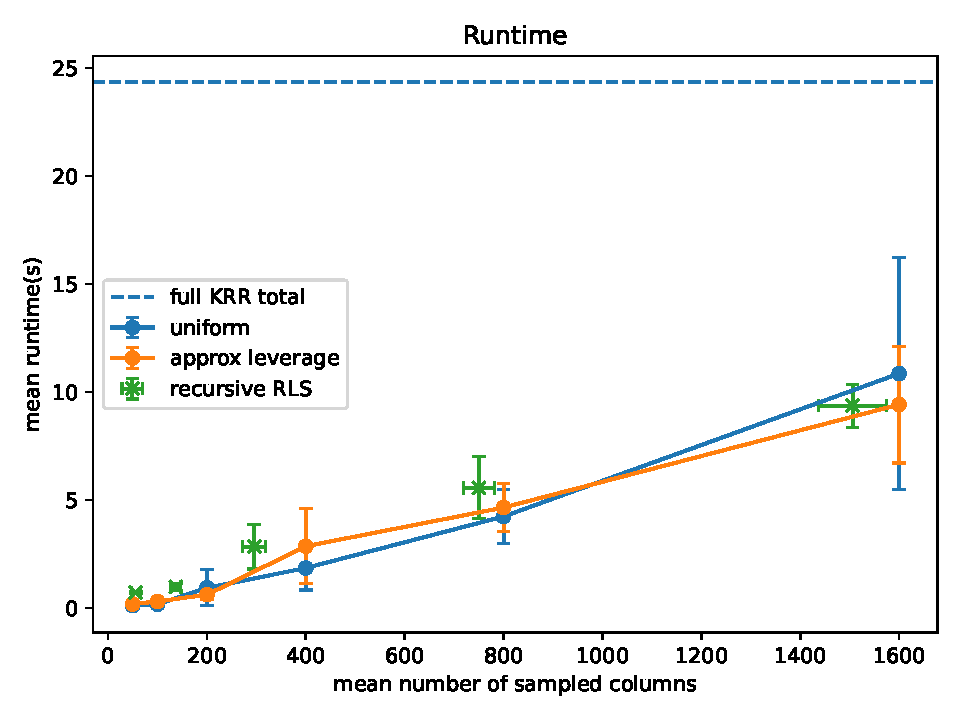
\includegraphics[width=0.98\textwidth]{Results/Superconductivityfinal_total_time_vs_l.pdf}
\caption{Mean total runtime against mean $l$.}
\label{fig:ftt}
\end{minipage}
\end{figure}
\FloatBarrier

Figure \ref{fig:fst} shows that uniform sampling is essentially free, and approximate leverage sampling only adds a small cost. Recursive RLS has a larger sampling cost which looks approximately linear with the number of columns, but this is not the main bottleneck at large column counts compared to the solve time since all methods have similar total times at large $l$. Figure \ref{fig:ftt} shows the total runtime. It rises quickly as $l$ increases and becomes a substantial fraction of the full KRR total reference time at the largest fixed column count. This shows that optimizing the sampling step alone may not be enough to reduce the overall runtime. However, at the smaller recursive samples, the recursive sampling step can still form a substantial fraction of the total runtime while uniform sampling remains essentially free.

For example, with $\lambda_{\mathrm{RLS}}=1000$, recursive RLS selected a mean of $1506$ columns with a standard deviation of approximately $68$ columns. Its mean sampling time was approximately $2.36$ seconds, while the common solve after column sampling took approximately $7.01$ seconds, giving a mean total runtime of approximately $9.37$ seconds. The full KRR total reference time was approximately $24.34$ seconds, consisting of approximately $6.37$ seconds for full kernel construction and $17.97$ seconds for the dense solve and test prediction. Recursive Nystr\"om was therefore approximately $2.6$ times faster overall at this point, while having approximately $6\%$ relative excess test RMSE. However, the common solve still formed about three quarters of its Nystr\"om runtime, showing that this solver becomes the main Nystr\"om bottleneck at large $l$. Therefore, the solver is efficient when $l\ll n$, which means that Nystr\"om approximation helps most if the sampling method keeps $l$ genuinely small.

\begin{figure}[H]
\centering
\begin{minipage}{0.49\textwidth}
\centering
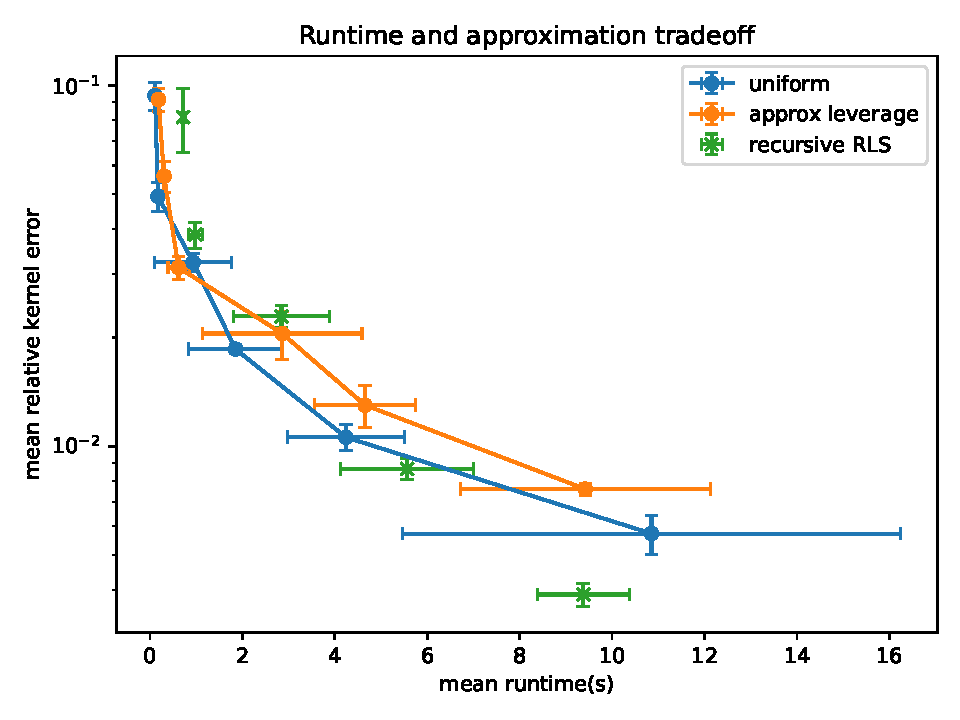
\includegraphics[width=0.98\textwidth]{Results/Superconductivityfinal_runtime_kernel_error_tradeoff.pdf}
\caption{Mean runtime and kernel approximation error.}
\label{fig:frke}
\end{minipage}
\hspace{0.005\textwidth}
\begin{minipage}{0.49\textwidth}
\centering
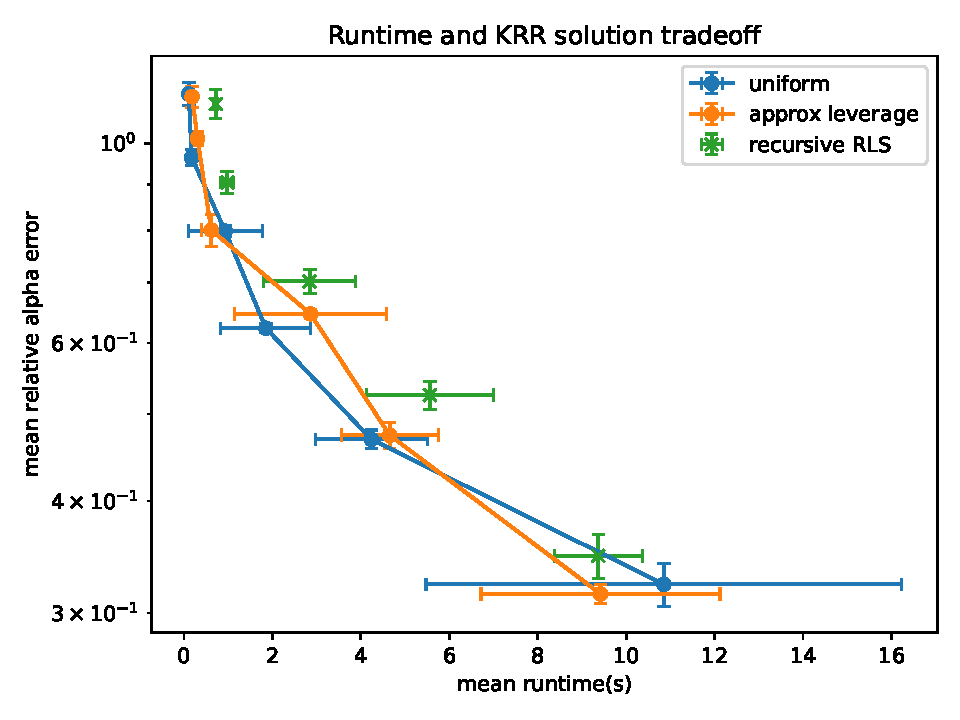
\includegraphics[width=0.98\textwidth]{Results/Superconductivityfinal_runtime_alpha_error_tradeoff.pdf}
\caption{Mean runtime and coefficient error.}
\label{fig:frae}
\end{minipage}
\end{figure}
\FloatBarrier

Figures \ref{fig:frke} and \ref{fig:frae} show the same general trade off at the matrix and coefficient levels, runtime increases generally give better approximations. Recursive RLS seems to achieve a smaller kernel approximation error at a similar runtime, but this does not produce the same clear advantage in coefficient error or test RMSE. Therefore a slightly better approximation of $K$ does not automatically give a better prediction runtime trade off.

\section{Secondary results and residual diagnostics}

The next figures check whether the approximation and the solver behave consistently. They are not the central results but they can show whether large errors come from the solver failing or from the approximation losing important information.

\begin{figure}[H]
\centering
\begin{minipage}{0.49\textwidth}
\centering
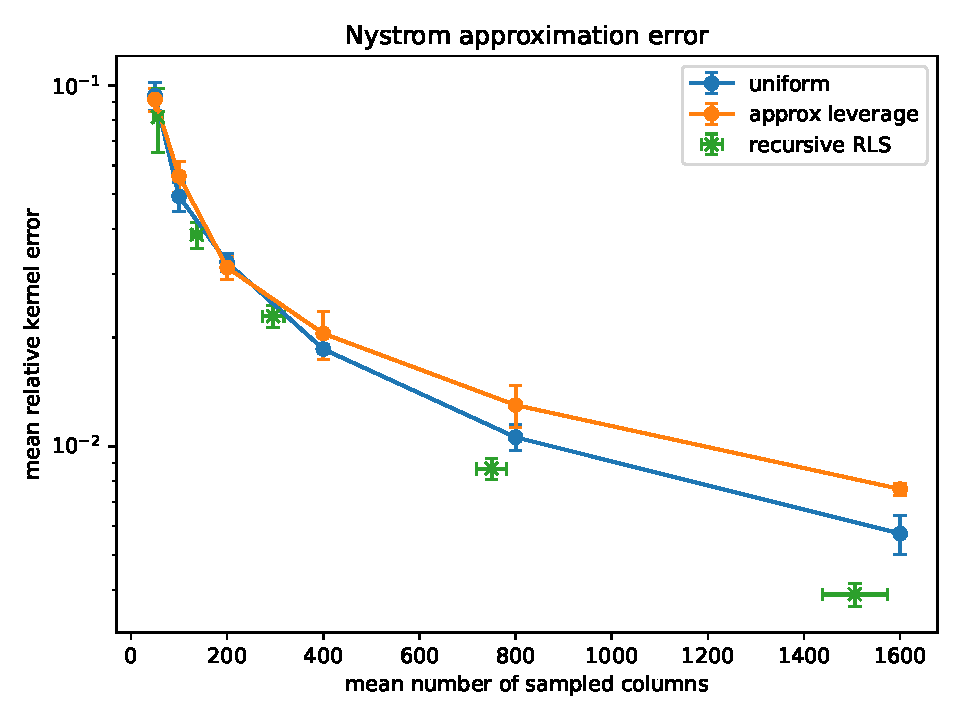
\includegraphics[width=0.98\textwidth]{Results/Superconductivityfinal_kernel_error_vs_l.pdf}
\caption{Mean relative kernel error.}
\label{fig:fkevl}
\end{minipage}
\hspace{0.005\textwidth}
\begin{minipage}{0.49\textwidth}
\centering
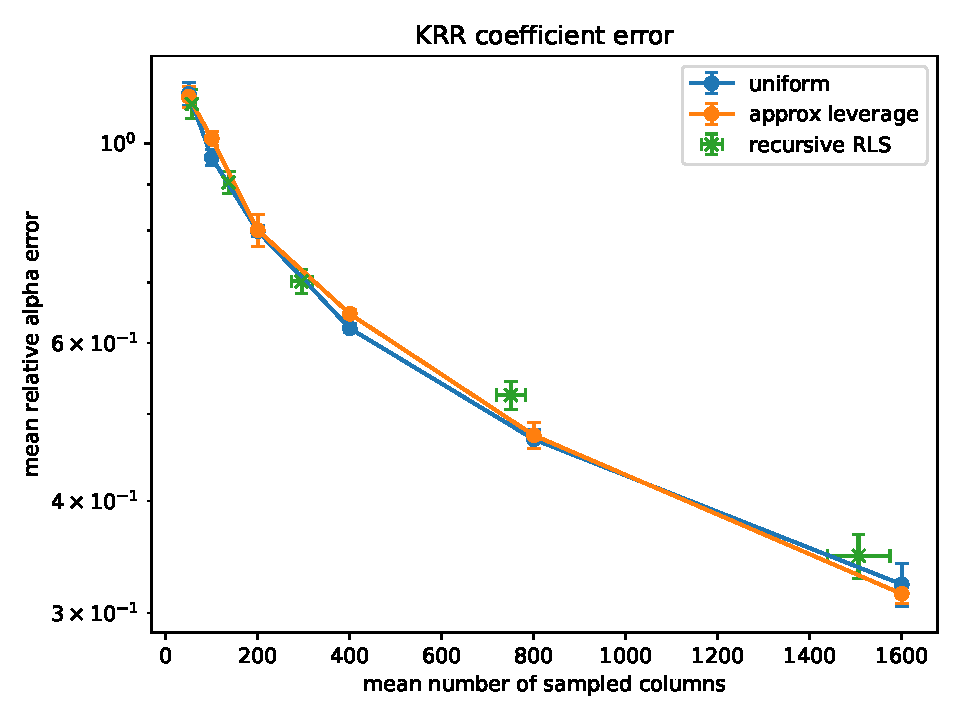
\includegraphics[width=0.98\textwidth]{Results/Superconductivityfinal_alpha_error_vs_l.pdf}
\caption{Mean relative KRR coefficient error.}
\label{fig:faevl}
\end{minipage}
\end{figure}
\FloatBarrier

Figure \ref{fig:fkevl} shows that the direct matrix approximation error decreases with $l$. Recursive RLS can have very small kernel error when it selects enough columns. At a mean of $1506$ columns, its mean relative kernel error is approximately $0.0039$, compared with approximately $0.0057$ for uniform sampling and $0.0076$ for approximate leverage sampling at $l=1600$. Figure \ref{fig:faevl} shows similar behavior, however, recursive RLS does not have the smallest coefficient error at these large column counts. Thus the ordering of the methods by kernel approximation error does not necessarily match their ordering by coefficient error.

The residual diagnostics below come from a representative single run rather than the five run averages. They are kept because their purpose is to validate the solver rather than to compare the expected performance of sampling methods.

\begin{figure}[H]
\centering
\begin{minipage}{0.49\textwidth}
\centering
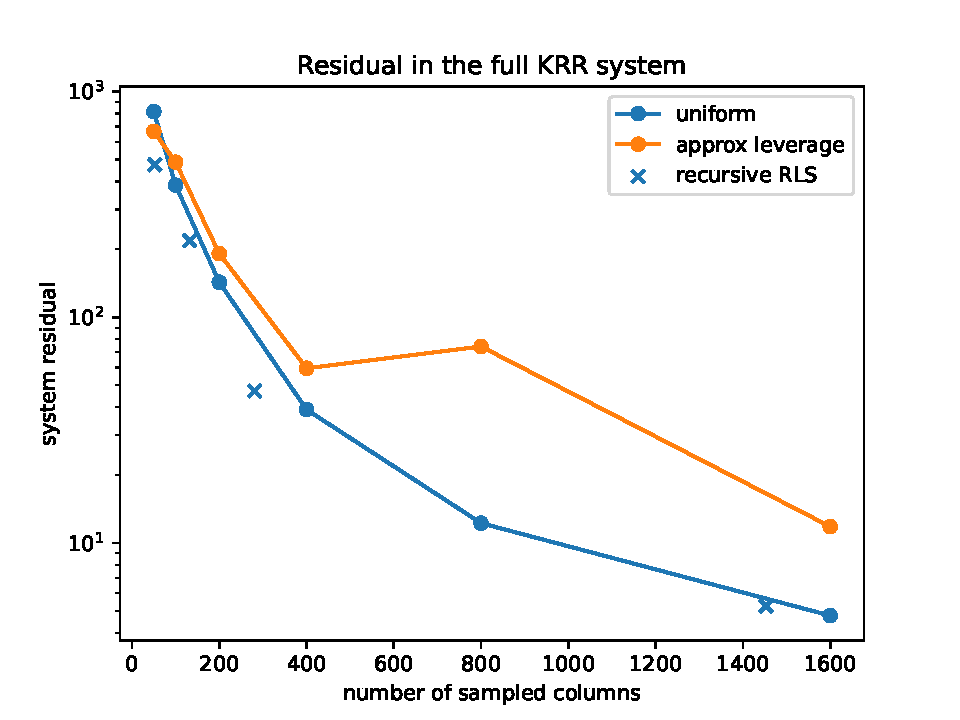
\includegraphics[width=0.98\textwidth]{Results/final_full_system_residual_vs_l.pdf}
\caption{Residual in the full KRR system for a representative run.}
\label{fig:ffl}
\end{minipage}
\hspace{0.005\textwidth}
\begin{minipage}{0.49\textwidth}
\centering
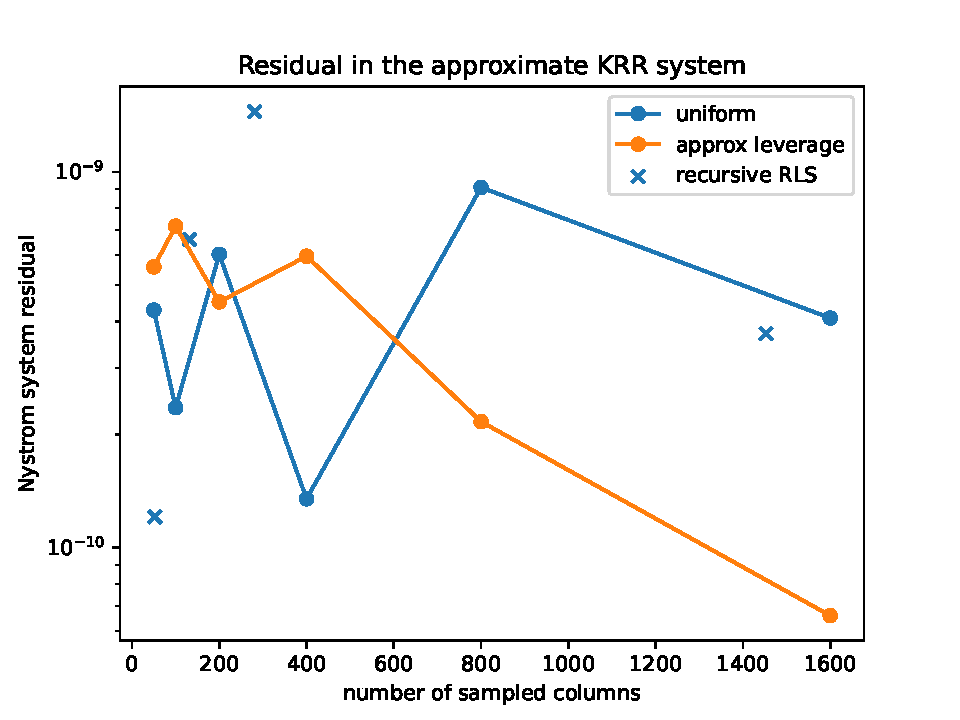
\includegraphics[width=0.98\textwidth]{Results/final_nystrom_system_residual_vs_l.pdf}
\caption{Residual in the approximate Nystr\"om system for a representative run.}
\label{fig:fnsl}
\end{minipage}
\end{figure}
\FloatBarrier

Figure \ref{fig:ffl} inserts the approximate solution into the original full system and measures
\[
\frac{\|(K+\lambda_{\mathrm{KRR}}I)\tilde\alpha-y\|_2}{\|y\|_2}.
\]
This residual decreases as the approximation improves, but it is not close to zero. That is as expected since $\tilde\alpha$ solves the approximate system instead of the full system. Figure \ref{fig:fnsl} measures the residual in the approximate system
\[
\frac{\|(\tilde K+\lambda_{\mathrm{KRR}}I)\tilde\alpha-y\|_2}{\|y\|_2}.
\]
These residuals are very small. Therefore the solver is doing what it should and it solves the approximate Nystr\"om system accurately. The remaining error comes from replacing $K$ by $\tilde K$ instead of a numerical failure of the solve.

\section{Repeated experiments on additional datasets}\label{sec:additional_datasets}

To determine whether the behaviour observed for Superconductivity is specific to one kernel matrix, the same five repetition experiment was carried out on the CASP protein structure dataset and the CT Slice Localization dataset \citep{physicochemical_properties_of_protein_tertiary_structure_265, relative_location_of_ct_slices_on_axial_axis_206}. We repeated the exact same set up as the main dataset and obtained the following.

\begin{figure}[H]
\centering
\begin{minipage}{0.49\textwidth}
\centering
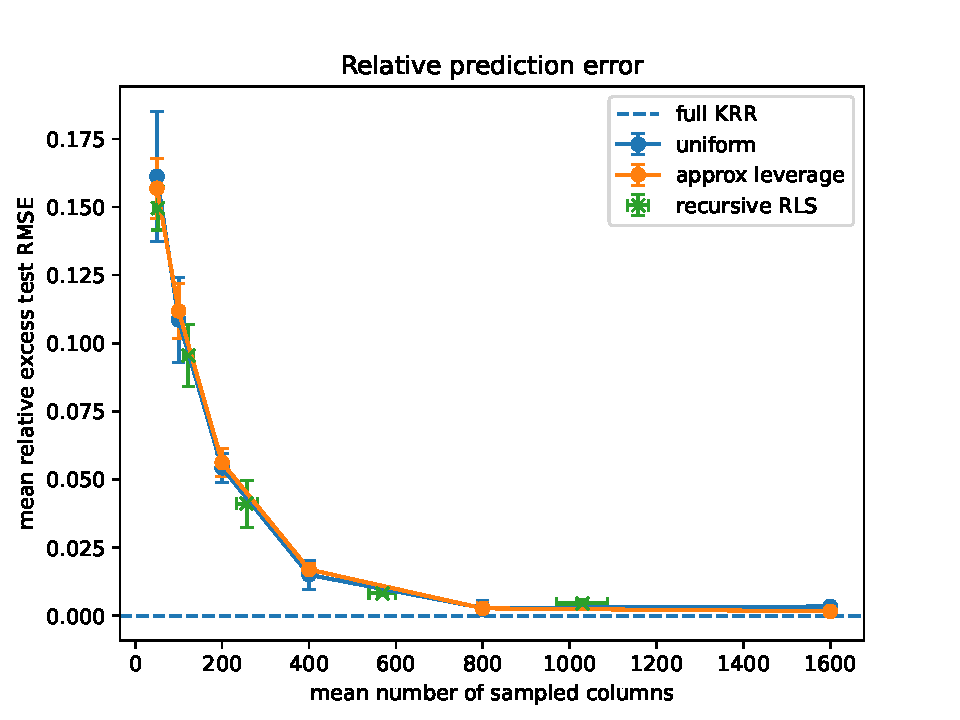
\includegraphics[width=0.98\textwidth]{Results/CASPfinal_relative_excess_rmse_vs_l.pdf}
\caption{Mean relative excess test RMSE for CASP.}
\label{fig:crr}
\end{minipage}
\hspace{0.005\textwidth}
\begin{minipage}{0.49\textwidth}
\centering
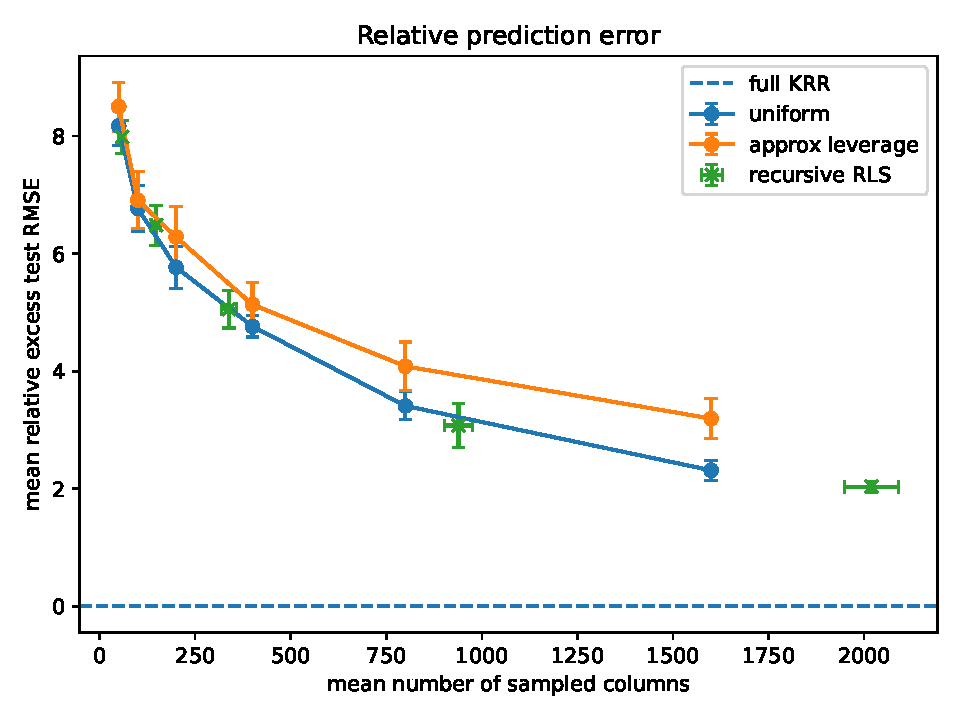
\includegraphics[width=0.98\textwidth]{Results/CTSliceLocalizationfinal_relative_excess_rmse_vs_l.pdf}
\caption{Mean relative excess test RMSE for CT Slice Localization.}
\label{fig:ctrr}
\end{minipage}
\end{figure}
\FloatBarrier

The two datasets show the same general pattern as the main dataset, increasing the number of landmarks generally improves prediction accuracy. However the methods remain very close on CASP while clearer differences seem to be present at larger column counts on CT Slice Localization. Moreover, the rate at which the predictions of all methods approach full KRR differs substantially between the datasets.

Figure \ref{fig:crr} shows that CASP converges much faster than Superconductivity. Uniform sampling has approximately $1.5\%$ relative excess RMSE at $l=400$ and approximately $0.3\%$ at $l=800$. The other two sampling methods give almost the same result. Therefore CASP reaches the full KRR prediction region with substantially fewer columns than Superconductivity.

Figure \ref{fig:ctrr} shows the opposite case. CT Slice Localization improves as $l$ increases, but it does not approach full KRR over the tested range. At $l=1600$, uniform sampling still has approximately $231\%$ relative excess RMSE and approximate leverage sampling approximately $320\%$. Recursive RLS has approximately $203\%$ relative excess RMSE even when it returns a mean of approximately $2020$ columns. It seems that we would need a lot more columns to reduce the error further. Superconductivity therefore lies between the rapidly converging CASP case and the much more slowly converging CT Slice Localization case.

The previous figures compare prediction accuracy at a given number of sampled columns. However, to compare the practical trade off directly, Figure \ref{fig:crt} and \ref{fig:ctrt} plot the relative excess test RMSE against the mean total runtime of each Nystr\"om method.
 
\begin{figure}[H]
\centering
\begin{minipage}{0.49\textwidth}
\centering
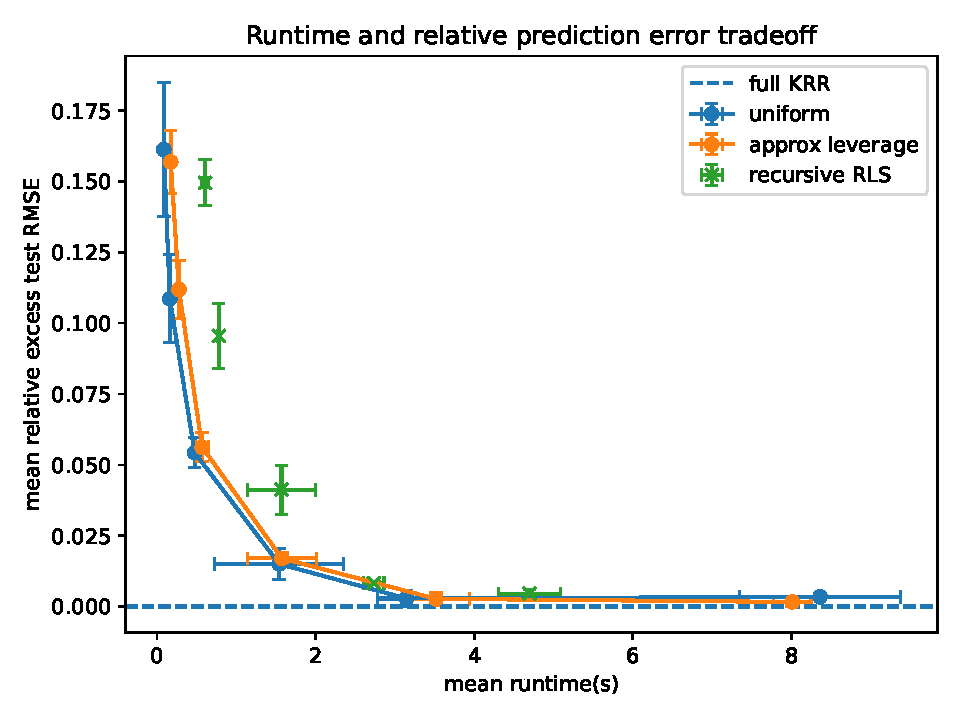
\includegraphics[width=0.98\textwidth]{Results/CASPfinal_runtime_relative_excess_rmse_tradeoff.pdf}
\caption{Mean runtime and relative excess test RMSE for CASP.}
\label{fig:crt}
\end{minipage}
\hspace{0.005\textwidth}
\begin{minipage}{0.49\textwidth}
\centering
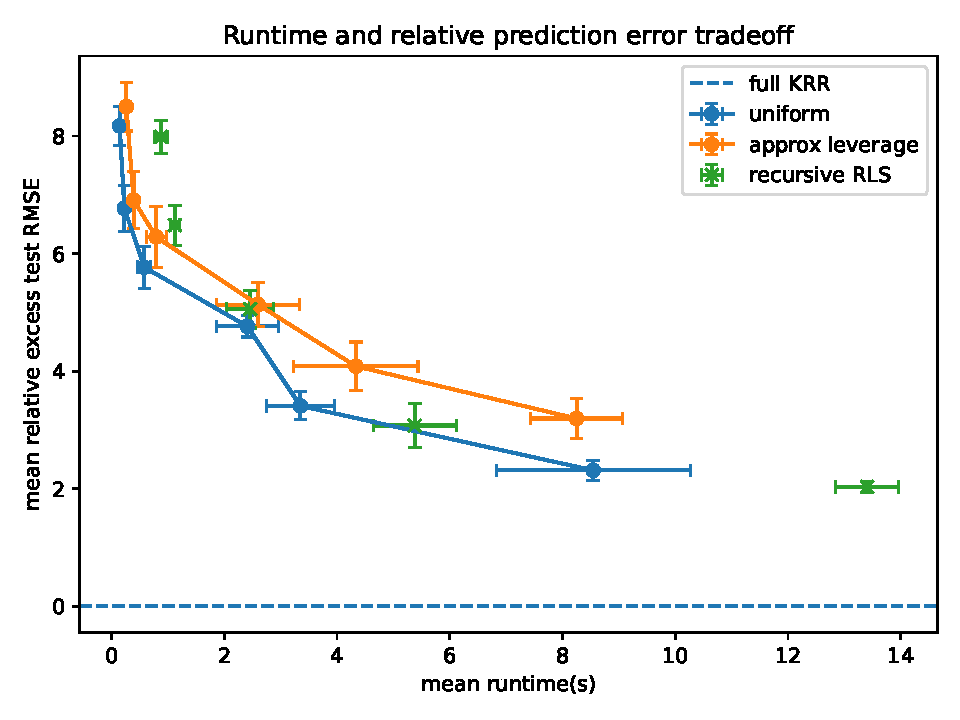
\includegraphics[width=0.98\textwidth]{Results/CTSliceLocalizationfinal_runtime_relative_excess_rmse_tradeoff.pdf}
\caption{Mean runtime and relative excess test RMSE for CT Slice Localization.}
\label{fig:ctrt}
\end{minipage}
\end{figure}
\FloatBarrier

Uniform and approximate leverage sampling remain close on CASP with recursive RLS slightly worse at low column count. However, approximate leverage sampling performs worse than uniform sampling at the larger landmark counts on CT Slice Localization. Recursive RLS does not provide a consistent prediction advantage across the datasets. These results strengthen the earlier conclusion that a more informed sampling strategy does not automatically produce a better prediction runtime trade off.

To investigate why the three datasets require different numbers of columns, the eigenvalues of fixed $2000\times2000$ kernel submatrices were compared. This was repeated across different $n$s which all gave the same pattern. The figure below shows a controlled spectral comparison without requiring the complete eigendecomposition of each $19000\times19000$ kernel matrix.

\begin{figure}[H]
\centering
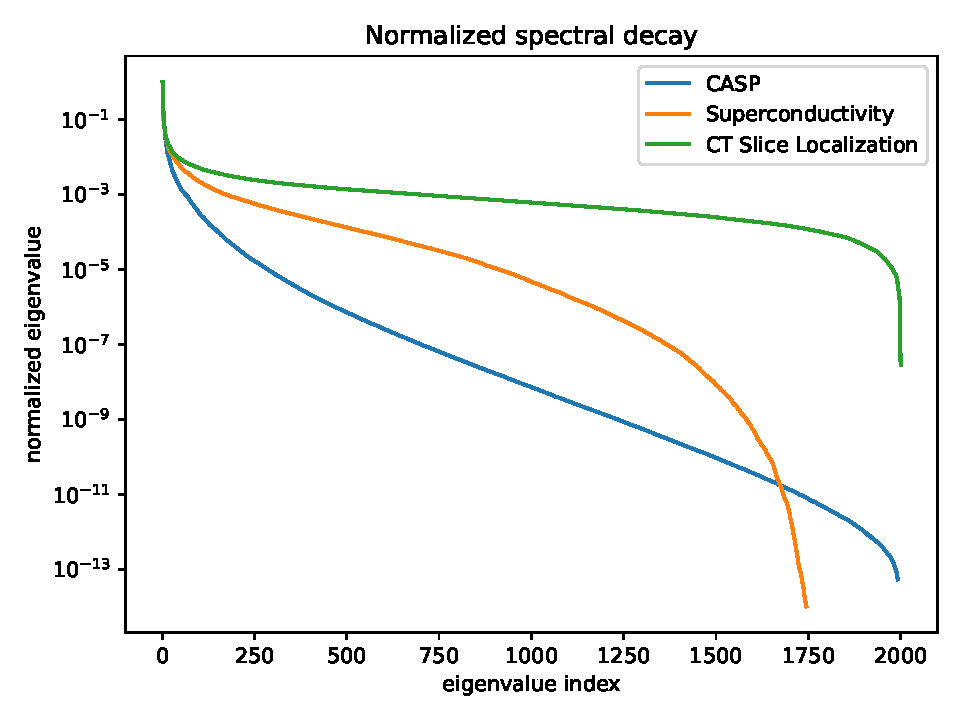
\includegraphics[width=0.78\textwidth]{Results/cross_dataset_normalised_spectrum.pdf}
\caption{Normalized eigenvalue decay for $2000\times2000$ kernel submatrices.}
\label{fig:cds}
\end{figure}
\FloatBarrier

Figure~\ref{fig:cds} shows that the CASP eigenvalues decay the fastest, the Superconductivity eigenvalues have an intermediate decay, and the CT Slice Localization eigenvalues decay slowest.

The relative spectral decay is consistent with the prediction curves. The faster decay for CASP is consistent with its requiring relatively few landmarks, while the slower decay for CT Slice Localization is consistent with its much slower approach to full KRR. Since the eigenvalues are normalized, this figure gives a qualitative spectral explanation rather than directly showing how many directions are important at $\lambda_{\mathrm{KRR}}=0.01$.

This does not mean that spectral decay is the only reason for the differences between the datasets. However, this gives a reasonable explanation for why the required landmark count is dataset dependent. The additional experiments therefore show that the improvement with increasing $l$ is stable across datasets, but the number of columns required to approach full KRR can vary significantly across different kernel matrices.